\documentclass[10pt]{article}
\usepackage[utf8]{inputenc}
\usepackage[T1]{fontenc}
\usepackage{amsmath}
\usepackage{amsfonts}
\usepackage{amssymb}
\usepackage[version=4]{mhchem}
\usepackage{stmaryrd}
\usepackage{graphicx}
\usepackage[export]{adjustbox}
\graphicspath{ {./images/} }
\usepackage{caption}

%New command to display footnote whose markers will always be hidden
\let\svthefootnote\thefootnote
\newcommand\blfootnotetext[1]{%
  \let\thefootnote\relax\footnote{#1}%
  \addtocounter{footnote}{-1}%
  \let\thefootnote\svthefootnote%
}

%Overriding the \footnotetext command to hide the marker if its value is `0`
\let\svfootnotetext\footnotetext
\renewcommand\footnotetext[2][?]{%
  \if\relax#1\relax%
    \ifnum\value{footnote}=0\blfootnotetext{#2}\else\svfootnotetext{#2}\fi%
  \else%
    \if?#1\ifnum\value{footnote}=0\blfootnotetext{#2}\else\svfootnotetext{#2}\fi%
    \else\svfootnotetext[#1]{#2}\fi%
  \fi
}

\begin{document}

\section*{5 Flaring protoplanetary disk (10 Points)}
Planets are the products of collapsing clouds forming circumstellar disks around the young stars. In this problem, we examine the thermal structure of a type of protoplanetary disks. We consider radiation from the central star to be the dominant heating process and assume that the disk is optically thick and the radiation can be only absorbed in the surface layers of the disk. This type of disk is called a flaring disk (see figure 1 below). In this case, the star illuminates the surface of the disk directly, and the shallow angle $\beta$ between the light rays and the surface of the disk increases with distance from the star.\\
(a) Find an expression for $\beta$ as a function of $r$. Assume $h(r) \ll r$.

Hint: the expression involves $h(r), r$ and $\frac{\Delta h(r)}{\Delta r}$\\
(b) Find an expression for the equilibrium temperature of the disk ( $T_{D}$ ) as a function of $\beta(r), r$ and luminosity $\left(L_{s}\right)$ of the star (Ignore the size of the star).\\
(c) We parameterize the disc height as $h(r)=a r^{b}$, where $a$ and $b$ are constants. For which values of $a$ and $b$ is the condition for an isothermal layer ( $T_{D}=$ Constant) satisfied? Write your answer for constant $a$ in terms of $T_{D}$ and $L_{S}$

Hint: If $\Delta r \ll r$, then $\left(1+\frac{\Delta r}{r}\right)^{b} \approx 1+\frac{b \Delta r}{r}$.

\begin{figure}[h]
\begin{center}
  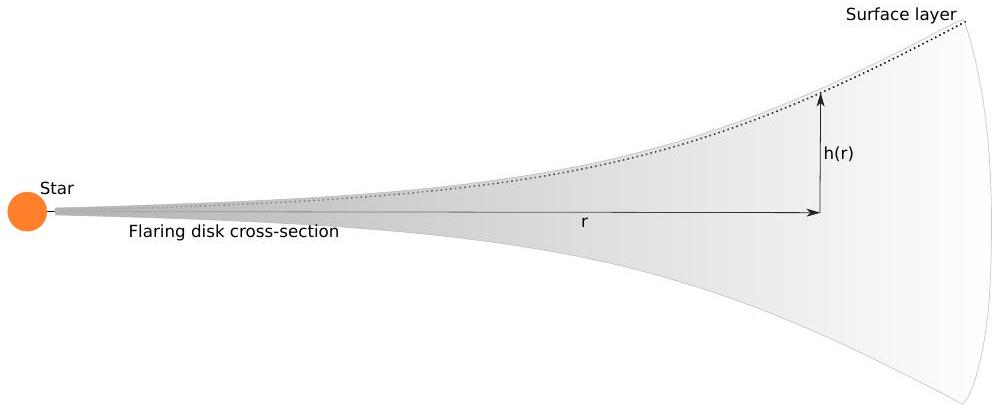
\includegraphics[width=\textwidth]{2025_09_11_6312450c103d6a7e5736g-03}
\captionsetup{labelformat=empty}
\caption{Figure 1: cross section of flaring disk}
\end{center}
\end{figure}

\end{document}